% Chapter ComecocosWeb
\chapter{Comecocos Web} % Main chapter title
\section{Enunciado}
En la actualidad gracias a las novedades introducidas en la Web han aumentando los juego desarrollado sin la necesidad de puglins o software de terceros para su ejecución.
\\Por ello en esta primera practica se pide desarrollar un juego con herramientas nativas de la web.Dentro de las varias opciones existentes el juego seleccionado es Pac-Man(comecocos).
\begin{figure}[!h]
\begin{center}
   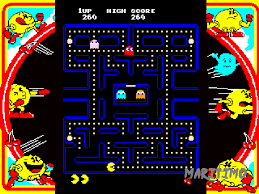
\includegraphics[width=0.5\linewidth]{Figures/Pacman_Intro}
	\decoRule
	\caption[Aspecto clásico Pacman]{Aspecto clásico Pacman.}
\label{fig:Pacman_Intro}
\end{center}
\end{figure}
\subsection{Requisitos}
Se presenta los distintos elemento que forman parte del juego y la función que deben desarrollar.
\begin{enumerate}
\item \textbf{Escenario:} Contiene todos los elementos estáticos del juego con los que interactua Pacman como pueden ser los obstáculos y el contorno del escenario que no pueden ser sobrepasados y los cocos que es la comida de Pacman.Ademas informara al usuario del tiempo y puntos a medida que progrese la partida.
\item \textbf{Pacman:} se trata del personaje principal del juego que controle el usuario.
\item \textbf{Fantasmas:} son los enemigos que persiguen a Pacman durante la partida.En total serán 4 fantasmas\footnote{fuente:\url{http://gameinternals.com/post/2072558330/understanding-pac-man-ghost-behavior}} que ha diferencia de Pacman no interactuan con los elementos del juego ya que solo basan su comportamiento en la posición de Pacman,esto es conocido como modo de persecución por lo es necesario aplicar un algoritmo básico de Inteligencia Artificial.
\end{enumerate}
\subsection{Tecnologías necesarias}
\begin{enumerate}
\item HTML5 tags: canvas,audio.
\item HTML5 API: LocalStorage
\item JavaScript
\item Inteligencia Artificial.
\end{enumerate}
\section{Desarrollo}
Como se ha dicho a lo largo de este desarrollo la lógica del juego recae sobre JavaScript. Por esto se han creado tres tipos de objetos (GameArea, Pacman, Ghost) con el objetivo de hacer más compacto el código y menos repetitivo ya que hay muchas funciones que tienden a repetirse.
\subsection{Game Area}
Este objeto es el encargado de generar y dibujar los elementos del  juego. El objeto inicializa una serie de variables que hacen referencia a dichos elementos.
\begin{lstlisting}[
caption=Iniciacion de variables del Obj.Game]
  value_cuad : 40,
  filas:19,
  columnas:18,
  canvas : document.createElement("canvas"),
  image :new Image(),
  img_loose : new Image(),
  img_win : new Image(),
  /* time */
  seconds : 0,
  min : 0,
  horas :0,
  time : '00'+':'+'00'+':'+'00',
  state : 0,
  score :0,
  start_crono : false,
  lifePlayer : 1,
  shape_1 : [...
  ],
  shape_2 : [...
  ],
  list_cocos : [...
  ],
  list_obstaculos : [...
  ],
  var map: [...
  ]
\end{lstlisting}
Tras la creación de las variables es necesario dotar al objeto de una serie de funciones que permitan dibujar los elementos.
\subsubsection*{Start}
Inicializa el tamaño del lienzo y obtiene el contexto de \textit{canvas} para poder dibujar los elementos dentro de el. Ademas obtenemos la referencia a las imágenes y fuentes de audio que vamos a utilizar.
\begin{lstlisting}[
caption=Iniciacion de variables del Obj.Game]
 start : function() {
  this.img_loose.src ='game_over.jpeg';
  this.img_win.src = 'game_win.jpg';
  this.image.src = 'pacman_fruit.png';
  this.canvas.width = this.value_cuad*this.filas;
  this.canvas.height = this.value_cuad*(this.columnas+4);
  this.context = this.canvas.getContext("2d");
  document.body.insertBefore(this.canvas, 
  document.body.childNodes[2]);
  this.AudioGame =  document.getElementById('musica');
  this.AudioDied = document.getElementById('hitPacman');
  this.AudioEat = document.getElementById('eating');
 },
\end{lstlisting}
\subsubsection*{Escenario y elementos}
La función \textbf{shape\_scene} dibuja el escenario del juego por medio de un array con los comandos que se necesitan ejecutar.
\begin{lstlisting}[
caption=Visualizacion escenario.]
 shape_scene : function(shape){
  this.context.save();
  this.context.beginPath();
  for (var i = 0; i < shape.length; i++) {
   var elemento = shape[i];
   for (var propiedad in elemento){
    var x = elemento[propiedad];
    if(x.moveTo){
     this.context.moveTo(this.value_cuad*x.moveTo[0],
       this.value_cuad*x.moveTo[1]);
    }else if(x.lineTo){
     this.context.lineTo(x.lineTo[0]*this.value_cuad,
       this.value_cuad*x.lineTo[1]);
     }
    }
   }
   this.context.strokeStyle = 'blue';
   this.context.lineWidth = 2;
   this.context.stroke();
   this.context.restore();
   },
},
\end{lstlisting}
Para dibujar los obstáculos definimos la función \textbf{draw\_obstacles} que lee el contenido de la variable \textbf{list\_obstaculos}. Cada elemento esta formado por las coordenadas y dimensiones que se multiplican por el tamaño que tiene cada cuadro del escenario.
\begin{lstlisting}[
caption= Visualizacion obstaculos.]
 draw_obstacles : function(){
   for(var i=0;i<this.list_obstaculos.length;i++){
    var elemento = this.list_obstaculos[i]; 
     this.context.fillRect(elemento.x*value_cuad,elemento.y*value_cuad,
       elemento.width*value_cuad,elemento.height*value_cuad);
   }
},
\end{lstlisting}
Los últimos elementos son los cocos que por medio de la función \textbf{ draw\_doits} se dibujan. La función lee el contenido de la variable \textbf{list\_cocos}, donde cada elemento tiene la misma estructura que los elementos de la variable \textbf{list\_obstaculos}.
\begin{lstlisting}[
caption=Visualizacion cocos.]
 draw_doits : function(){
  if(this.list_cocos.length > 0){ 
   for(var i=0;i<this.list_cocos.length;i++){ 
    var elemento = this.list_cocos[i]; 
    this.context.fillStyle = 'white'; 
    this.context.beginPath(); 
    this.context.arc((elemento.x*40)+20,(elemento.y*40)+20,
       elemento.radio,0,(Math.PI/180),true);
    this.context.fill();
   }
 }
},
\end{lstlisting}
En la imagen \ref{fig:ElementosGame} se muestra el aspecto que tiene el escenario al utilizar las funciones anteriores.
\begin{figure}[!h]
\begin{center}
   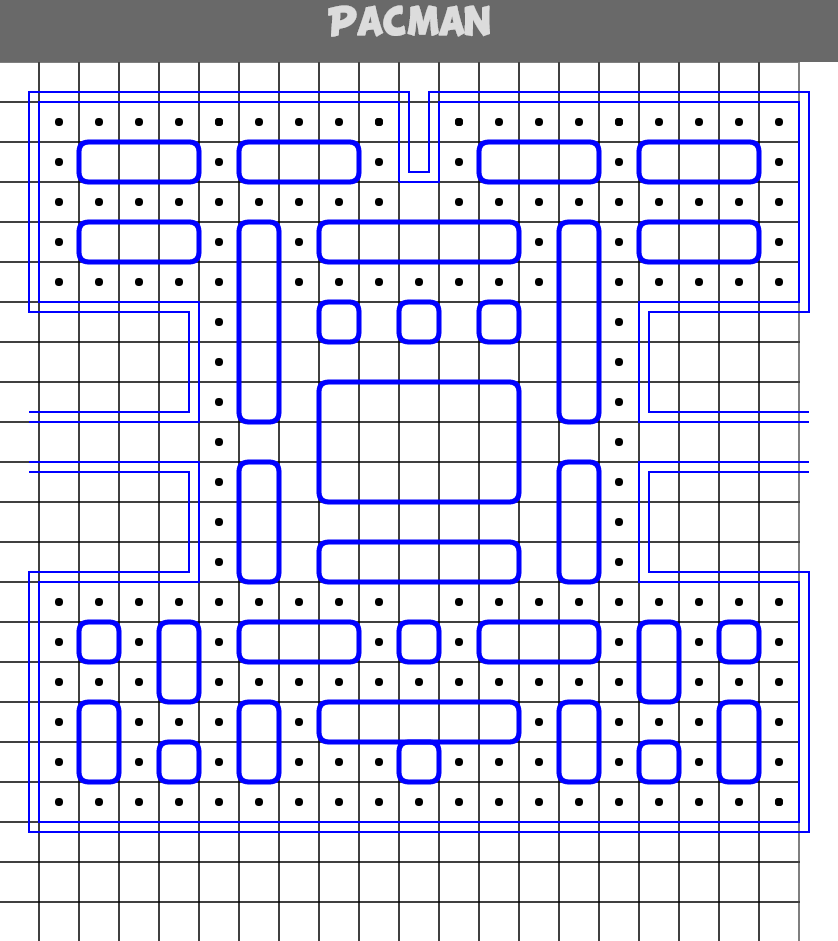
\includegraphics[width=0.4\linewidth]{Figures/ElementosGame}
	\decoRule
	\caption[Apariencia elementos del juego]{Apariencia elementos del juego.}
\label{fig:ElementosGame}
\end{center}
\end{figure}
\subsubsection*{Información de la partida}
Otra característica que presenta el objeto es mostrar información sobre el estado de la partida.
\\La función \textbf{time\_game} se encarga de dibujar el cronometro del juego. Para ello dibuja el valor que contiene la variable \textbf{time}.El valor de esta variable se actualiza por medio de la función \textbf{CronoTime} que se explica mas adelante.
\begin{lstlisting}[
caption=Visualizacion cronometro.]
 time_game:function(){
  this.context.save();
  this.context.font = "30px BDCartoonShoutRegular";	
  roundedRect(this.context,8*40,20*40,5*40,1*40,10);
  this.context.fillStyle = "#00FA9A";
  this.context.fillText(this.time,8.75*40,20.80*40);
  this.context.restore();
 },
 \end{lstlisting}
También dibuja la información del marcador del usuario por medio de la función \textbf{score\_user} que utiliza la información de variable \textbf{score}.
\begin{lstlisting}[
caption=Visualizacion Marcador.]
 score_user : function(){
  this.context.save();
  this.context.fillStyle = "white";
  this.context.font = "30px BDCartoonShoutRegular";
  this.context.fillText('score: '+this.score,1*40,20*40);
  this.context.restore();
 },
\end{lstlisting} 
Por ultimo, la función \textbf{life\_user} se encarga de dibujar el contenido de la variable \textbf{life}.
\begin{lstlisting}[
caption=Visualizacion vidas.]
 life_user : function(){
  this.context.save();
  this.context.fillStyle = "white";
  this.context.font = "30px BDCartoonShoutRegular";
  this.context.fillText('life: '+this.life,1*40,21*40);
  this.context.restore();
 },
\end{lstlisting}
En la imagen \ref{fig:InfoGame} se muestra el aspecto que tiene el escenario al utilizar las funciones anteriores.
\begin{figure}[!h]
\begin{center}
   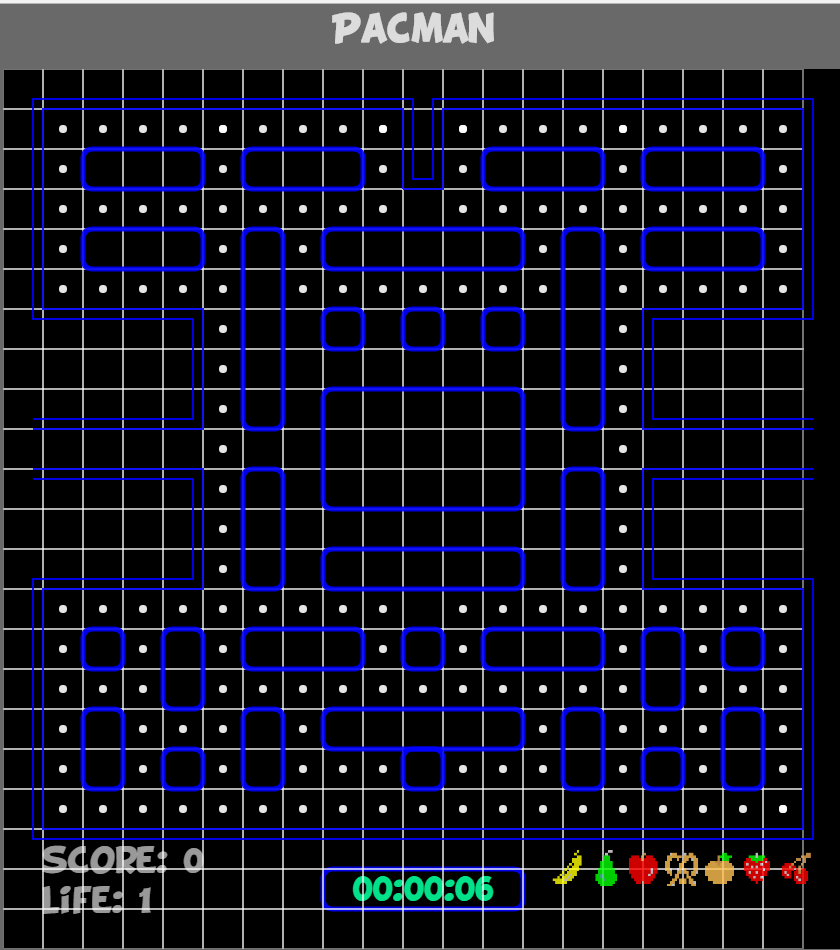
\includegraphics[width=0.4\linewidth]{Figures/InfoGame}
	\decoRule
	\caption[Apariencia información del juego]{Apariencia información del juego.}
\label{fig:InfoGame}
\end{center}
\end{figure}
\subsubsection*{Fin de Partida}
La partida puede terminar cuando Pacman ha logrado comerse todos los cocos de la partida lo que produce la ejecución de la función \textbf{win\_game} que carga una imagen indicando al usuario que ha ganado y permite guardar la información de la partida a través de una función \textbf{PosMouseClick} que se explica mas adelante.
\begin{lstlisting}[
caption=Visualizacion Partida Ganada.]
win_game : function(){
  var finish = false;
  if(this.list_cocos == 0){
    this.context.globalAlpha = 0.9;
    this.context.save();
    this.context.drawImage(this.img_win,0,0,
      this.canvas.width,this.canvas.height);
    roundedRect(this.context,this.canvas.width/2-(4*40),13*40,
      8*40,1.5*40,10);
    this.context.fillStyle = "#00FA9A";
    this.context.font = "30px BDCartoonShoutRegular";
    this.context.fillText('Save Score',
      this.canvas.width/2-(2.5*40),14*40);
    this.context.restore();
    finish = true;
   }
  return finish
},
\end{lstlisting} 
Otro forma de terminar la partida se produce cuando los fantasmas capturan a Pacman lo que produce la ejecución de la función \textbf{lose\_game} que carga una imagen indicando al usuario que ha perdido.
\begin{lstlisting}[
caption=Visualizacion Partida Perdida.]
 lose_game : function(){
  this.context.save();
  this.context.globalAlpha = 0.6;	
  this.context.drawImage(this.img_loose,0,0,
    this.canvas.width,this.canvas.height);
  this.context.restore();
 },
\end{lstlisting} 
\subsection{Pacman}
Es el protagonista del juego y por ende el usuario interactúa con el moviéndolo por todo el
escenario. En su lógica tenemos que tener en cuenta diversos factores que afectan a su progreso
por el juego.
\subsubsection*{Detectar colisiones}
Tenemos que tener en cuenta el entorno del juego con respecto a la posición en la que se encuentra Pacman.Para ello la función \textbf{hitt\_Counter} evalúa que las coordenadas(x,y) no sobrepasen el contorno del escenario.
\begin{lstlisting}[
caption=Deteccion de colisiones con el escenario.]
 this.hitt_counter = function(){
  var hitt_counter = false;
   if(this.x < 0 || this.x > GameArea.filas){
    hitt_counter = true;
   }else if(this.y < 0 || this.y > GameArea.columnas){
    hitt_counter = true;
   }
   return hitt_counter;
 }
 \end{lstlisting}
Otro tipo de colisión a tener en cuenta es con los obstáculos, de esto se encarga la función \textbf{hitObject}.La función obtiene los vértices del objeto y de Pacman para comprobar si alguno de los vértices de Pacman se encuentran dentro del área que forman los vértices del objeto.
\begin{lstlisting}[
caption=Deteccion de colisiones con objetos del juego.]
 this.hitObject = function(list){
  var hitt = false;
  for(var i = 0;i<list.length;i++){
   var obstaculo = list[i];
   var Aobstaculo = {x:obstaculo.x,y:obstaculo.y};
   var Bobstaculo = {x:obstaculo.x+obstaculo.width,
       y:obstaculo.y};
   var Cobstaculo = {x:obstaculo.x,
       y:obstaculo.y+obstaculo.height};
   var Dobstaculo = {x:obstaculo.x+obstaculo.width,
       y:obstaculo.y+obstaculo.height};
   var Apac = {x:this.x,y:this.y};
   var Bpac = {x:this.x+this.width,y:this.y};
   var Cpac = {x:this.x,y:this.y+this.height};
   var Dpac = {x:this.x+this.width,y:this.y+this.height};
   if(Apac.x > Aobstaculo.x  && Apac.x < Bobstaculo.x &&
    Apac.y >  Aobstaculo.y && Apac.y < Cobstaculo.y){
    hitt = true;
    break
   }
   if(Bpac.x  >  Aobstaculo.x  && Bpac.x < Bobstaculo.x &&
    Bpac.y >  Aobstaculo.y && Bpac.y < Cobstaculo.y){
     hitt = true;
     break
   }
   if(Cpac.x >  Aobstaculo.x && Cpac.x < Bobstaculo.x && 
    Cpac.y >  Aobstaculo.y && Cpac.y < Cobstaculo.y){
     hitt = true;
     break
   }
   if(Dpac.x >   Aobstaculo.x && Dpac.x < Bobstaculo.x &&
    Dpac.y  >  Aobstaculo.y && Dpac.y <  Cobstaculo.y){
     hitt= true;
     break
   }
 }
 if(hitt == true){
  this.move = false;
 }
}
 \end{lstlisting}
En la imagen \ref{fig:ColisionObjetos} se muestra la colisión con un objeto impidiendo a Pacman avanzar.
\begin{figure}[!h]
\begin{center}
   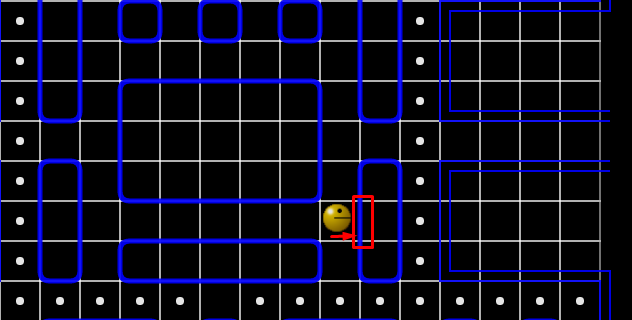
\includegraphics[width=0.5\linewidth]{Figures/ColisionObjetos}
	\decoRule
	\caption[Colisión Pacman-Obstáculo]{Colisión Pacman-Obstáculo.}
\label{fig:ColisionObjetos}
\end{center}
\end{figure}
\subsubsection*{Comer Cocos}
Los cocos se encuentran por todo el escenario por lo que es necesario comprobar si hay colisión con ellos. 
\\La función \textbf{eat\_doit} calcula los vértices de pacman para evaluar si la posición del coco esta dentro del área formada por los vértices anteriores.En caso afirmativo se elimina este elemento de la variable \textbf{GameArea.score} para no volverlo a ser dibujado.
\begin{lstlisting}[
caption=Detección de colisión con los cocos.]
 this.eat_doit = function(list_cocos){
  var eat = false;
  for(var i=0;i<list_cocos.length;i++){
   var coco = list_cocos[i];
   var Apac = {x:this.x,y:this.y};
   var Bpac = {x:this.x+this.width,y:this.y};
   var Cpac = {x:this.x,y:this.y+this.height};
   var Dpac = {x:this.x+this.width,y:this.y+this.height};
    if (coco.x+0.5 > Apac.x && coco.x+0.5 < Bpac.x && 
      coco.y+0.5 > Apac.y && coco.y+0.5 < Cpac.y ){
      list_cocos.splice(i,1);
      eat = true
      GameArea.score = GameArea.score +4 ;
      break;
    }
   }
   return eat;
 }
\end{lstlisting}
En la imagen \ref{fig:EatCoco1} se muestra la colisión con un coco lo que provoca que dicho coco desaparezca.
\begin{figure}[!h]
\begin{center}
   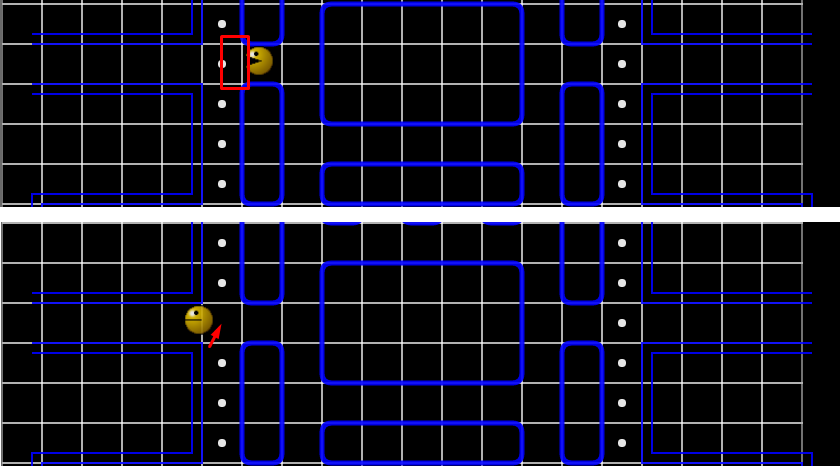
\includegraphics[width=0.5\linewidth]{Figures/EatCoco1}
	\decoRule
	\caption[Colisión Pacman-Cocos]{Colisión Pacman-Cocos.}
\label{fig:EatCoco1}
\end{center}
\end{figure}
\subsubsection*{Actualizar posición Canvas}
Para actualizar la posición de Pacman la función \textbf{new\_position} suma los nuevos valores que han sido asignados al haber pulsado una tecla en las variables \textbf{x\_speed} e \textbf{y\_speed}.
\begin{lstlisting}[
caption=Actualizar posición en canvas.]
 this.new_position = function (){
  this.x += this.speed_x;
  this.y += this.speed_y;
 }
 \end{lstlisting}
Tras esto, la función \textbf{add\_steps} actualiza el valor de la variable \textbf{pasos} que es un contador definido para evaluar si su valor es  +/-1 lo que indica que se ha desplazado a una nueva casilla del mapa.
\begin{lstlisting}[
 caption=Actualización de pasos dados.]
 this.add_steps = function(){
  if(this.speed_x != 0 || this.speed_y != 0){
   if(this.type_move == 'y_pos' || this.type_move == "y_neg"){
    this.pasos += this.speed_y;
   }else{
    this.pasos += this.speed_x;
   }
  }
 }
\end{lstlisting}
\subsubsection*{Actualizar posición Mapa}
Actualizamos el valor de las variables \textbf{x\_map} e \textbf{y\_map} según corresponda y restablecemos el valor de la variable \textbf{pasos}.
\begin{lstlisting}[
caption=Actualización coordenada del mapa.]
 this.new_path = function(){
  if(this.x_map < 22 && this.x_map >= 0){
   if(this.y_map < 19 && this.y_map >= 0){
    if(this.type_move == 'y_pos'){
      this.y_map += 1;	
    }else if(this.type_move == 'x_pos'){
      this.x_map += 1;
	}else if(this.type_move == 'y_neg'){
      this.y_map -= 1;
    }else{
      this.x_map -= 1;
	}
    this.pasos = 0;
    this.new_pos = true;	
    }
  }
 }
 \end{lstlisting}
\subsubsection*{Dibujar}
Finalmente, para dibujar a Pacman utilizamos la función \textbf{drawImagen()} de canvas que carga el trozo de imagen correspondiente a Pacman del spreedsheet.Posee dos estados de dibujo para crear la sensación de animación.
\begin{lstlisting}[
caption=Dibujar Pacman.]
 this.draw = function(){
  GameArea.context.save();
  if(this.state_draw == 0){
   GameArea.context.drawImage(this.image,320,this.yDraw,32,32
     ,this.x*40,this.y*40,35,35);
   this.state_draw = 1;
  }else{
  GameArea.context.drawImage(this.image,320+32,this.yDraw,
      32,32,this.x*40,this.y*40,35,35);
    this.state_draw = 0;
  }
  GameArea.context.restore();
 }
 \end{lstlisting}
\subsection{Fantasmas}
Definimos el objeto \textbf{Ghost} que tiene la lógica del comportamiento de los cuatro fantasmas que forman parte del juego.
\\En el momento de instanciar el objeto \textbf{Ghost(x\_map,y\_map,name,speed,initMoment)} le pasamos las coordenadas (x\_map,y\_map) donde se dibujara,el nombre,su velocidad y el numero de cocos que Pacman tiene que haber comido para salir a perseguirlo.
\subsubsection*{Persecución Pacman}
La función \textbf{init} se encarga de evaluar si se tiene que activar el fantasma, en caso afirmativo lo coloca fuera de la casa y empieza la persecución.
\begin{lstlisting}[
caption=Actualizar posicion del los Fantasmas.]
   this.init = function(score){
  	if(score == this.initMoment && !this.move){
     this.x_map =11;
     this.y_map =7;
     this.move = true;
  	}
  }
\end{lstlisting}
\subsubsection*{Actualizar objetivo}
La función \textbf{new\_path} aplica IA a cada fantasmas, por medio del mapa del juego obtiene el camino que cada fantasma tiene que seguir. Para ello tomamos como punto de inicio la posición actual del fantasma y la posición de Pacman formado por las variables x\_map e y\_map como punto de destino .A continuación explicamos el modo de persecución de cada fantasma.
\begin{itemize}
\item \textit{Blinky}: su comportamiento es seguir a Pacman en la misma dirección, entonces el punto de inicio es la posición actual de fantasma y el punto final es la posición actual de Pacman.
\item \textit{Speedy}: al igual que Blinky persigue a Pacman, pero tiene en cuenta su dirección. En este caso el cálculo se realiza tomando como punto de partida la posición de Speedy y se consulta la dirección de Pacman , al resultado le sumamos/restamos 4 posiciones según corresponda para obtener el punto final.
\item \textit{Clyde}: tiene dos tipos de comportamientos que dependen de la distancia entre él y Pacman, si dicha distancia es mayor a ocho sigue en modo persecución en caso contrario deja de seguirlo y se aleja de él tomando como nuevo objetivo una de las esquinas.
\end{itemize}
El resultado de cada operación se guarda en la variable \textbf{result} correspondiente.
\begin{lstlisting}[
caption=Actualizar direccion hacia el objetivo]
 this.new_path = function(graph,pacman_x,pacman_y,direccion){
  var start = graph.grid[this.x_map][this.y_map];
  if(this.name == 'blinky'){
   var end = graph.grid[pacman_x][pacman_y];
  }else if(this.name == 'speedy'){
   if(pacman_x+4 < 21 && direccion == 'x_pos'){
    pacman_x += 4;
   }else if(pacman_x-4 > 0 && direccion == 'x_neg'){
    pacman_x -= 4;
   }else if(pacman_y+4 < 19 && direccion == 'y_pos'){
    pacman_y += 4;
   }else if(pacman_y-4 > 0 && direccion == 'y_neg'){
    pacman_y -= 4;
   }
   var end = graph.grid[pacman_x][pacman_y];
  }else if (this.name == 'clyde'){
   var end = graph.grid[pacman_x][pacman_y];
   this.result = astar.search(graph,start,end,false);
   if(this.result.length < 8){
   var end = graph.grid[this.cuad_static.x][this.cuad_static.y];
   }
  }
  this.result = astar.search(graph,start,end,false);
 }
\end{lstlisting}
\subsubsection*{Actualizar posición}
Para actualizar la posición de los fantasma vinculamos la función \textbf{nexStepGhost} por medio de un \textbf{timer} de forma que dicha función se ejecute según el valor definido en la variable \textbf{speed} de cada fantasmas.
\begin{lstlisting}[
caption=Actualizar posicion del los Fantasmas.]
 function nexStepGhost(ghost){
 ghost.flag = 1;
 if(ghost.result.length > 0){
  ghost.x = ghost.result[0].x;
  ghost.y = ghost.result[0].y;
  ghost.x_map = ghost.result[0].x;
  ghost.y_map = ghost.result[0].y;
  ghost.result.splice(0,1);
 }
 ghost.interval = setTimeout(function(){
  nexStepGhost(ghost)
  },ghost.speed);
 }
\end{lstlisting}
\subsubsection*{Dibujar}
Para dibujar los fantasmas lo hacemos igual que Pacman, pero al tener diferentes fantasmas por medio del nombre asignado en su creación obtenemos la imagen correspondiente a cada uno. 
\begin{lstlisting}[
caption=Dibujar Fantasma.]
 this.draw = function(){
  GameArea.context.save();
   if(this.name == 'blinky'){
    if(this.state_draw == 0){
     GameArea.context.drawImage(this.image,0,0,32,32,this.x_map*40,this.y_map*40,35,35);
    }else{
     GameArea.context.drawImage(this.image,32,0,32,32,this.x_map*40,this.y_map*40,35,35);
    }		
   }else if(this.name == 'clyde'){
    if(this.state_draw == 0){
     GameArea.context.drawImage(this.image,64,0,32,32,this.x_map*40,this.y_map*40,35,35);
    }else{
     GameArea.context.drawImage(this.image,94,0,32,32,this.x_map*40,this.y_map*40,35,35);
    }
   }else if(this.name == 'inky'){
    if(this.state_draw == 0){
     GameArea.context.drawImage(this.image,192,0,32,32,this.x_map*40,this.y_map*40,35,35);
    }else{
     GameArea.context.drawImage(this.image,222,0,32,32,this.x_map*40,this.y_map*40,35,35);
    }
    }else if(this.name == 'speedy'){
     if(this.state_draw == 0){
      GameArea.context.drawImage(this.image,128,0,32,32,this.x_map*40,this.y_map*40,35,35);
     }else{
      GameArea.context.drawImage(this.image,160,0,32,32,this.x_map*40,this.y_map*40,35,35);
     }
    }
    this.state_draw = ( this.state_draw === 1 ) ? 0 : 1;
    GameArea.context.restore();
  }
\end{lstlisting}
En la imagen \ref{fig:DrawGhost} se muestra un ejemplo del comportamiento de los fantasmas..
\begin{figure}[!h]
\centering
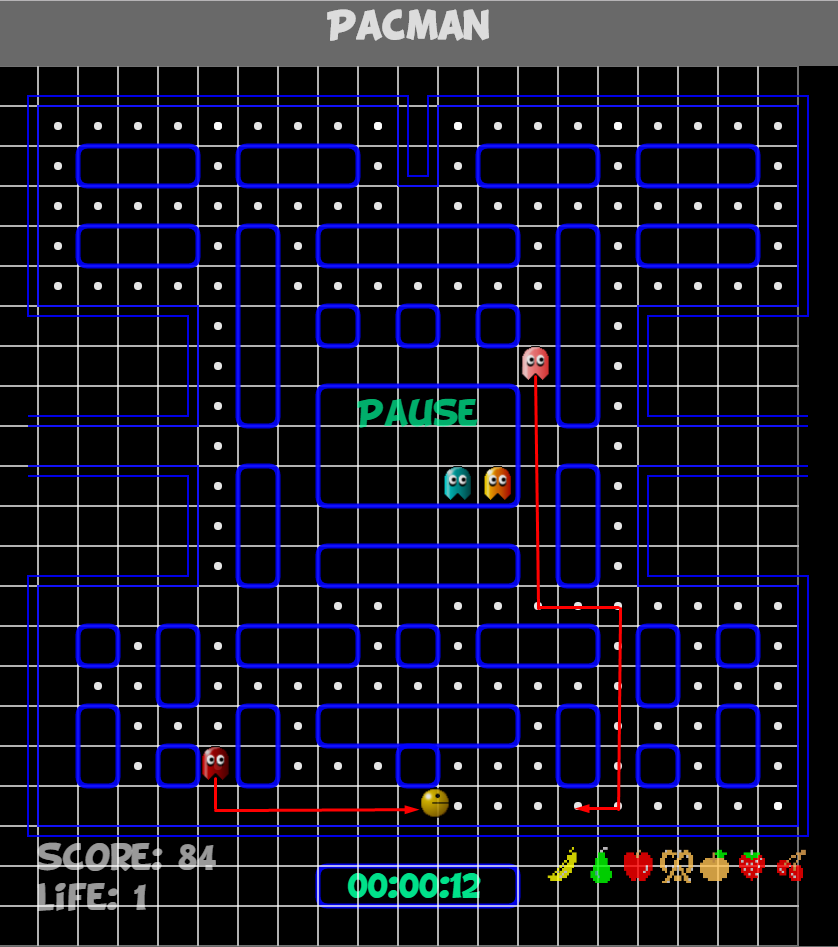
\includegraphics[width=0.4\linewidth]{Figures/SeguimientoGhost}
\decoRule
\caption[Apariencia comportamiento Fantasmas]{Apariencia comportamiento Fantasmas.}
\label{fig:DrawGhost}
\end{figure}
\subsection{Movimiento}
Para dotar de movimiento al juego a la función \textbf{updateGameArea} se vincula a un timer que se ejecuta cada 100ms y de esta forma mostrar las cambios de cada objeto.
\begin{lstlisting}[
caption=Renderizado del juego.]
 function updateGameArea(){
  /**  GameArea **/   
  GameArea.clear();
  GameArea.AudioGame.play();
  GameArea.time_game();
  GameArea.score_user();
  GameArea.life_user();
  GameArea.shape_scene();
  GameArea.draw_doits(list_cocos);
  GameArea.draw_obstacles(list_obstaculos);
  GameArea.draw_fruit();
 /** Fantasma **/
  for(var i = 0; i < list_Ghost.length;i++){
   var _ghost = list_Ghost[i];
   _ghost.init(GameArea.score);
   if(_ghost.move ){
    _ghost.new_path(graph,Pac.x_map,Pac.y_map,Pac.type_move);
   }
  }
  _ghost.draw();
  /** Pacman **/
  Pac.new_position();
  Pac.hitObject(list_Ghost);
  if(!Pac.move){
   /*Refibujamos todo el conteido del canvas diciendo que a perdido */
   GameArea.AudioGame.pause();
   GameArea.context.globalAlpha = 0.9;
   GameArea.context.save();
   GameArea.lose_game();
   GameArea.context.restore();
   GameArea.AudioDied.play();
   GameArea.stop();
  }else{
   var x = Pac.hitt_counter();
   Pac.hitObject(list_obstaculos);
   if(Pac.move != true || x == true){
    /* si hay choque hay que resetear el contenido para dibujar */
    Pac.reset();
   }else{
    Pac.add_steps();
    if(Pac.pasos == 1 || Pac.pasos == -1 ){
     Pac.new_path();
    }
   }
  }
  /* se comprueba si hemos comido algo para poner el sonido*/
  var eatPil = Pac.eat_doit(list_cocos);
  if(eatPil){
   GameArea.AudioGame.volume=0;
   GameArea.AudioEat.play();
   GameArea.AudioGame.volume=0;
  }
  Pac.reset_speed();
  Pac.draw();
  GameArea.win_game(list_cocos);
  if(list_cocos.length == 0){
   GameArea.stop();
  }
}
 \end{lstlisting}
\section{Pruebas}
El usuario  abre el archivo 'game\_pacman.html' dando lugar a la interpretacion del archivo por el navegador.
\begin{figure}[!h]
\centering
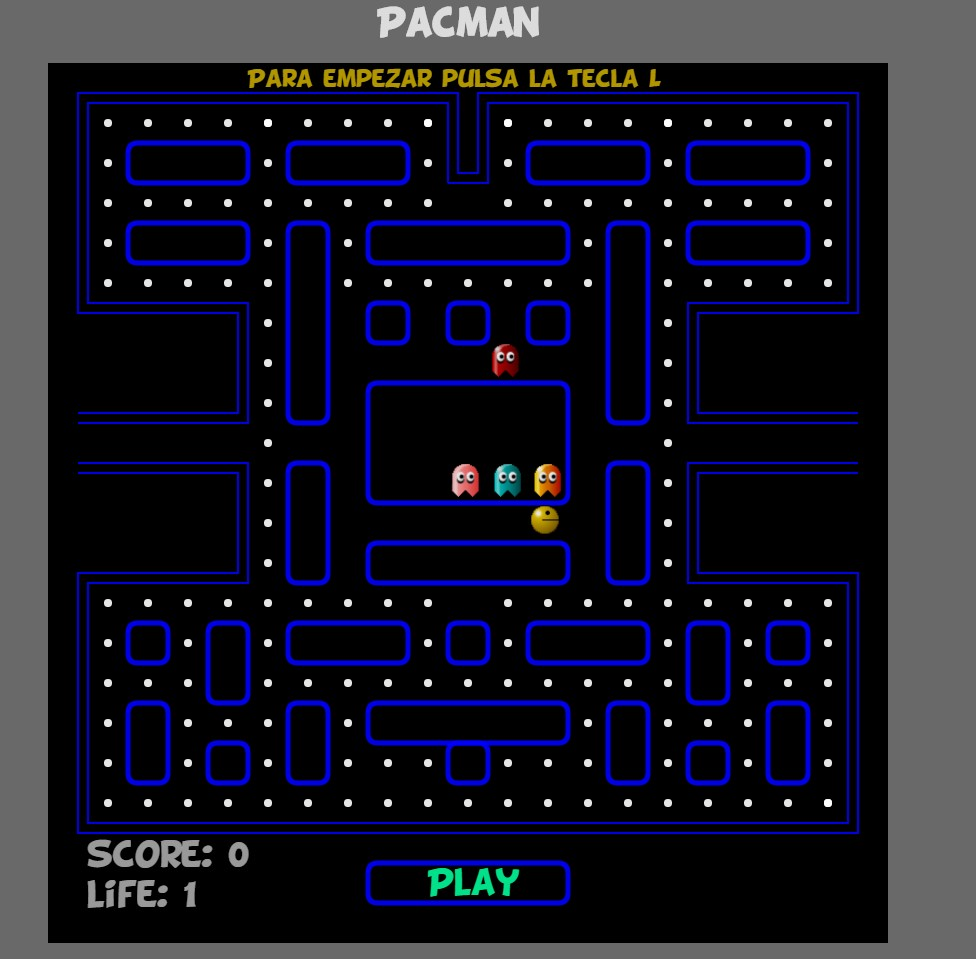
\includegraphics[width=80mm]{Figures/InitGame}
\decoRule
\caption[Inicio Juego]{Inicio juego Pacman.}
\label{fig:InitGame}
\end{figure}
Tras la interpretacion se muestra el escenario de juego con sus elementos y un panel informativo con datos de la partida \ref{fig:InitGame}.
\\Para iniciar la aplicación el usuario pulsa la tecla 'L'  provocando el movimiento de los fantasmas y el inicio del cronometro.A partir de este momento el usuario puede manipular a Pacman a traves de las flechas del teclado ademas se permite al usuario parar el juego pulsado la tecla 'P' e iniciar nuevamente el juego con la tecla 'L' imagen\ref{fig:Pause/Start game}.
\begin{figure}[!h]
\centering
\subfigure[Juego pausado]{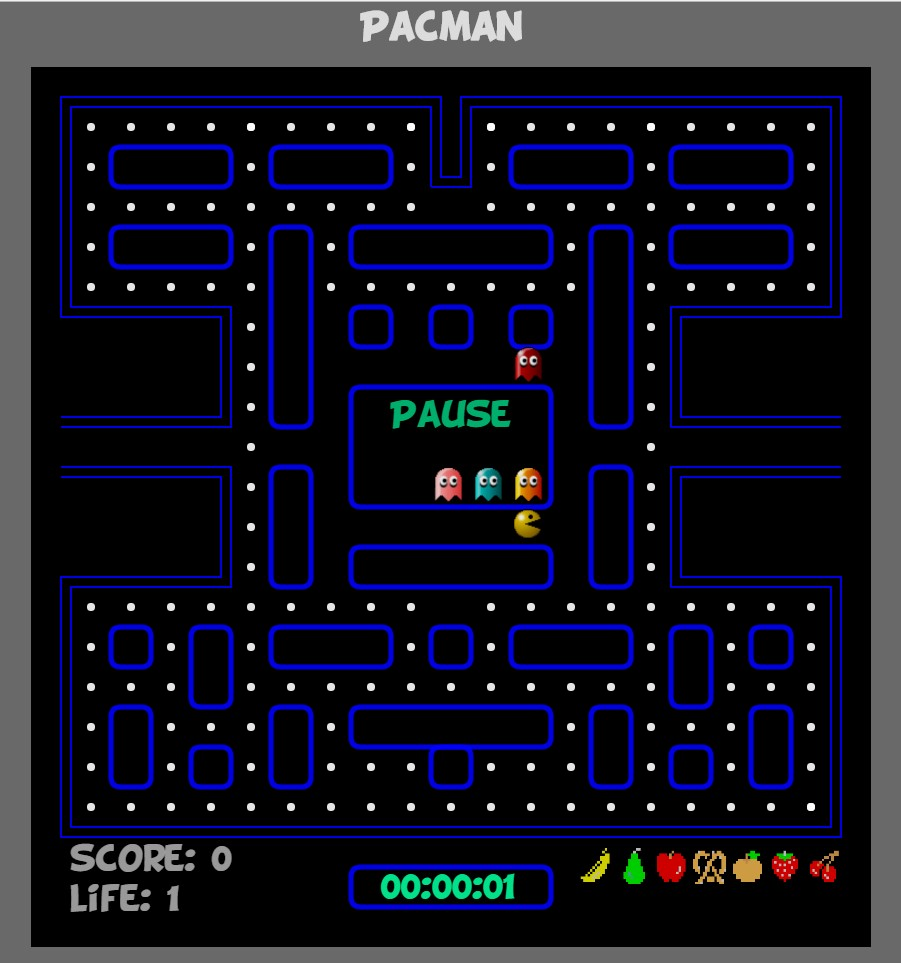
\includegraphics[width=43mm]{Figures/PauseGame}}\hspace{5mm}
\subfigure[Juego no pausado]{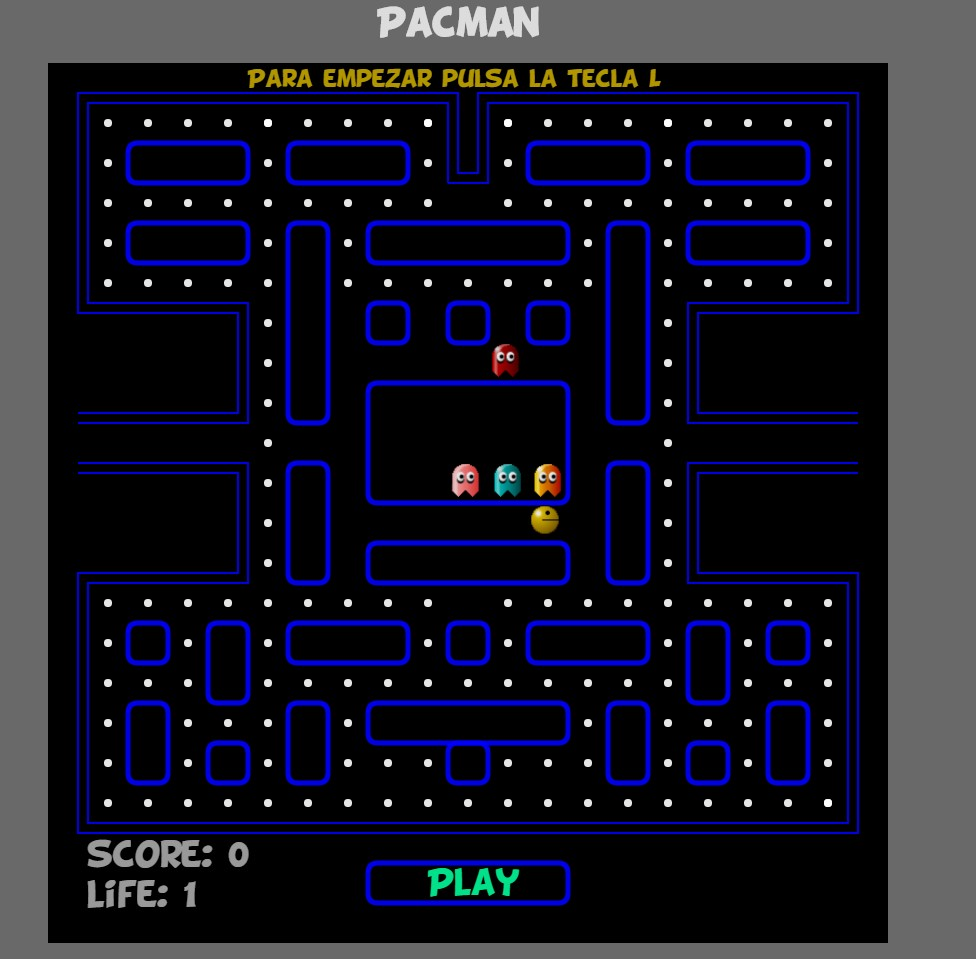
\includegraphics[width=43mm]{Figures/InitGame}}
\caption{Pause/Start juego.} \label{fig:Pause/Start game}
\end{figure}
\\Finalmente, el juego termina cuando se produce algunas de las situaciones que se mencionan a continuación  \ref{fig:Game/Loose game}
\begin{enumerate}
\item Cuando uno de los fantasmas atrapa a Pacman daremos la partida como perdida y en la pantalla se visualiza 'Game Over'.
\item Cuando Pacman se ha comido todos los cocos la partida finaliza la partida y el usuario ha ganado la partida. El usuario visualiza 'Win Game' y si quiere guardar informacion de la partida puede pulsar 'Save Score'.
\end{enumerate}
\begin{figure}[!h]
\centering
\subfigure[Partida perdida]{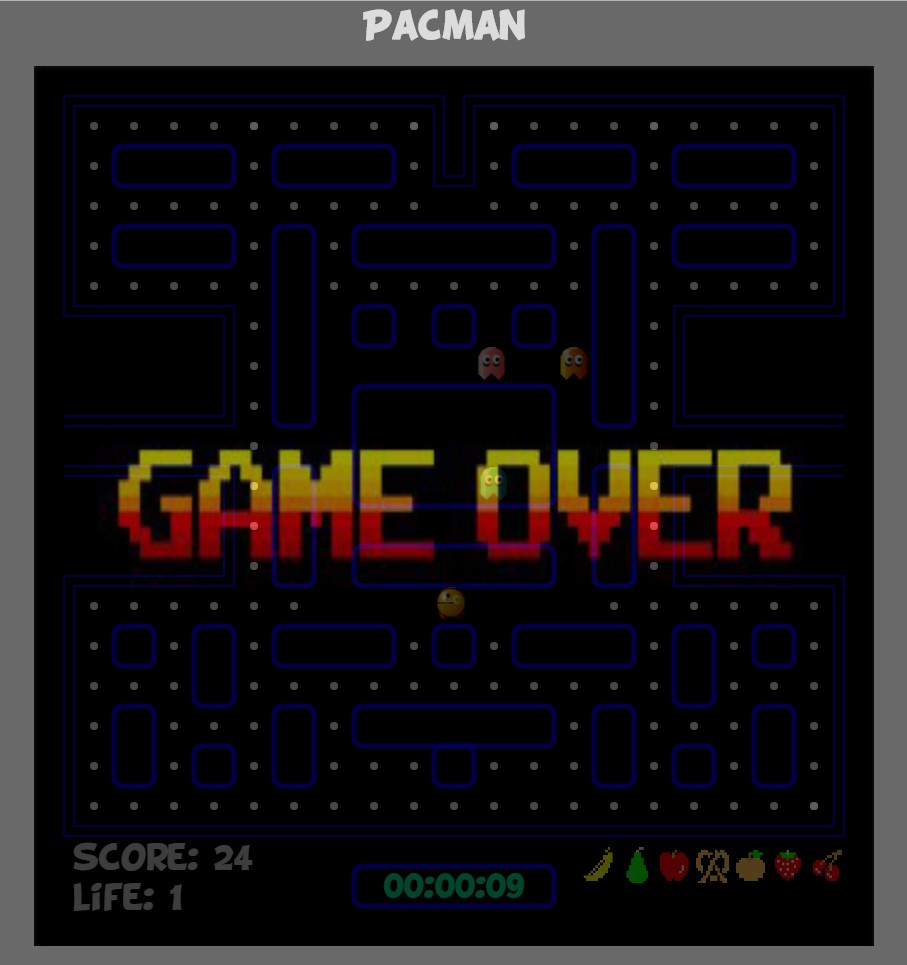
\includegraphics[width=40mm]{Figures/GameOver}}
\subfigure[Partida Ganada]{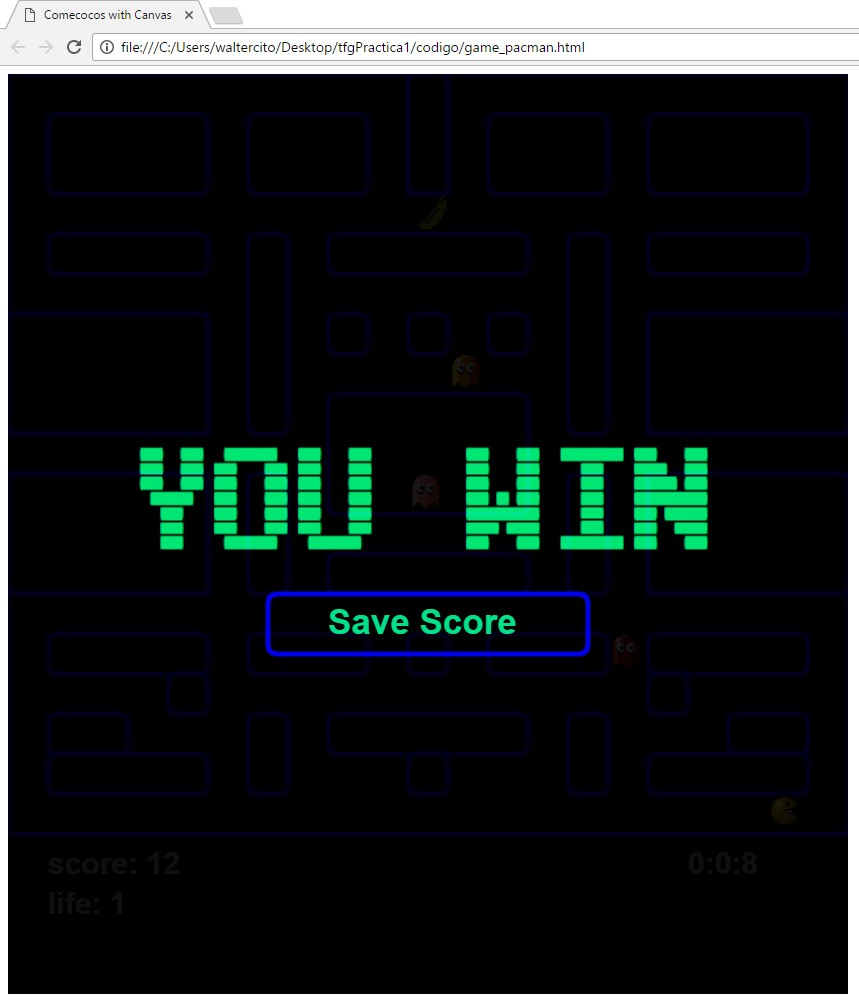
\includegraphics[width=40mm]{Figures/Win_Game}}
\caption{Game/Loose juego.} \label{fig:Game/Loose game}
\end{figure}
